

As mentioned previously, unlike Cartesian positions, the elements of orientation representations are constrained.
And these constraints need to be enocded in the the tranformation system of DMPs.

There are many ways in which the orientation are represented. In this work, we will use the quaternion representation.

\section{Quaternion Representation of DMP}
A quaternion or unit quaternion $\vect{q} = v + \vect{u}$ provides a representation of the orinetation of robots end effector, where The DMP equations for unit quaternion can be represented as:

\begin{align}
    \tau \vect{\dot{\eta}} &= \alpha_z(\beta_z * 2 * log(\vect{g_q} * \bar{\vect{q}}) - \vect{\eta}) + \vect{f_q(x)} \\
    \tau \vect{\dot{q}} &= \frac{1}{2} \vect{\eta} * \vect{q}
\end{align}
where, $\vect{g_q} \in \S^3 $ is the goal orientation, the quaternion conjugate is defined as $\vect{\bar{q}} = v - \vect{u}
\text{and} *$ denotes quaternion multiplication. $\eta$ is the scaled angular velocity $\omega$ and is
treated as unit quaternion with xero scalar component. The logaritminc mapping is defined as:

\begin{equation}
\log{\vect{q}} = 
\begin{dcases}
  \arccos{(v)} \ddfrac{\vect{u}}{||u||} &  \vect{u} \neq 0 \\
  0           &  \text{otherwise} 
\end{dcases}
\end{equation}

The above equations are based on the fact that the unit quaternion that takes $\vect{q_1}$ to $\vect{q_2}$
is given by $\Delta \vect{q} = \vect{q_2} * \vect{\bar{q_1}}$.Unlike with Rotation Matrices the logaritminc mapping defined on $\S^3$ has no discontinuity boundary, just a single singularity
at a sinlg e quaternion $\vect{q} = -1 + [0,0,0]^T $.

The nonlinear forcing term is defined similar to the standard discrete DMP, and is as follows:

\begin{equation}
    \vect{f_q(x)} = \ddfrac{\sum\limits_{i=1}^{N} w_i^o \Psi_i(x)}{\sum\limits_{i=1}^N \Psi_i(x)} = 
    \tau \vect{\dot{\eta}} - \alpha_z \left(  \beta_z * 2 * \log{ \left(  \vect{g_q} * \bar{\vect{q}}\right) } - \vect{\eta} \right)
\end{equation}
where, $w_i^0$ is the weights related to the orientation DMP, and like the discrete DMP can be solved using similar weight calculation methods.

To create a DMP system to reach a desired orientation, we created a orientation trajectory of quaternions using Spherical Liner Interpolation
(SLERP). In SLERP, the quaternions are interpolated using the following formula:

\begin{equation}
    \text{SLERP} = \vect{q_0} \left( \vect{q_0^{-1} q_1} \right)^t
\end{equation}
where $\vect{q_0}$ is the initial quaternion, $\vect{q_1}$ is the goal quaternion, and$\vect{q_0^-1 q_1}$ is 
the quaternion that takes the initial quaternion to the final quaternion. The results of the quaternion DMP where 
$\vect{q_0} =[0.70710678,0,-0.70710678,0] $  is interpolated to 
$\vect{q_g} = [0.37796447 , 0.75592895  ,0.37796447, -0.37796447]$ is shown below.

\begin{figure}[h]
\centering
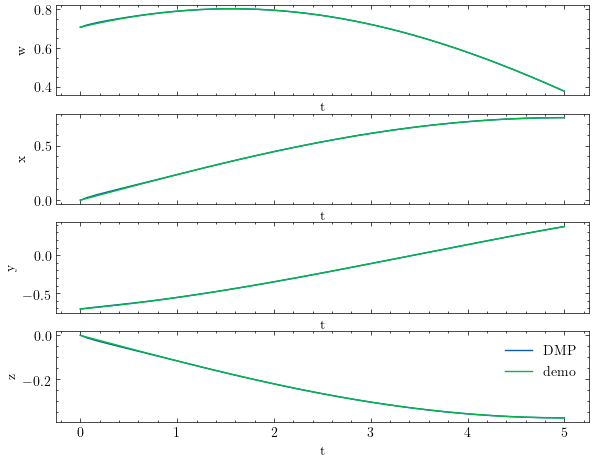
\includegraphics[width=0.7\textwidth]{quaternionDMP.png}
\caption{Quaternion DMP}
\label{fig:quaternionDMP}
\end{figure}




